%!TEX TS-program = xelatex
%  untitled
%
%  Created by David Rosenberg on 2009-09-10.
%  Copyright (c) 2009 University of Chicago. All rights reserved.
%
\documentclass[10pt,letterpaper]{article}
\usepackage{relsize,setspace}  % used by latex(describe( ))
\usepackage{hyperref,url}               % used in bibliography
\usepackage[superscript,nomove]{cite}
\usepackage{geometry}
% \usepackage{svn-multi}
% \svnidlong
% {$LastChangedDate: 2009-09-14 10:33:57 -0400 (Mon, 14 Sep 2009) $}
% {$LastChangedRevision: 6 $}
% {$LastChangedBy: root $}
% %\svnid{$Id: example_main.tex 146 2008-12-03 13:29:19Z martin $}
% % Don't forget to set the svn property 'svn:keywords' to
% % 'HeadURL LastChangedDate LastChangedRevision LastChangedBy' or
% % 'Id' or both depending if you use \svnidlong and/or \svnid
% %
% \newcommand{\svnfooter}{Last Changed Rev: \svnkw{LastChangedRevision}}
% \svnRegisterAuthor{root}{David M. Rosenberg}


\newcommand{\Reals}{\mathbb{R}}
\newcommand{\R}{\mathbb{R}}
\newcommand{\N}{\mathbb{N}}
\newcommand{\hreft}[1]{\href{#1}{\tt\small\url{#1}}}

\usepackage{fancyhdr}
\usepackage[parfill]{parskip}
\textwidth 6.5in
\pagestyle{fancy}
\newcommand{\bc}{\begin{center}}  % abbreviate
\newcommand{\ec}{\end{center}}
\newcommand{\code}[1]{{\smaller\texttt{#1}}}

% ----------------------------------------------------------------------------
\RequirePackage{fancyvrb}
\RequirePackage{listings}
% \usepackage{Sweave}
%
%----------------------------------------------------------------------------

%------------------------------------------------------------------------------
%------------------------------------------------------------------------------%
%Preparations for Sweave and Listings
%------------------------------------------------------------------------------%
%
\RequirePackage{color}
\definecolor{Rcolor}{rgb}{0, 0.5, 0.5}
\definecolor{RRecomdcolor}{rgb}{0, 0.6, 0.4}
\definecolor{Rbcolor}{rgb}{0, 0.6, 0.6}
\definecolor{Routcolor}{rgb}{0.461, 0.039, 0.102}
\definecolor{Rcommentcolor}{rgb}{0.101, 0.043, 0.432}
%------------------------------------------------------------------------------%
\lstdefinelanguage{Rd}[common]{TeX}%
{moretexcs={acronym,alias,arguments,author,bold,cite,%
          code,command,concept,cr,deqn,describe,%
          description,details,dfn,doctype,dots,%
          dontrun,dontshow,donttest,dQuote,%
          email,emph,enc,encoding,enumerate,env,eqn,%
          examples,file,format,item,itemize,kbd,keyword,%
          ldots,link,linkS4class,method,name,note,%
          option,pkg,preformatted,R,Rdopts,Rdversion,%
          references,S3method,S4method,Sexpr,samp,section,%
          seealso,source,sp,special,%
          sQuote,strong,synopsis,tab,tabular,testonly,%
          title,url,usage,value,var,verb},
   sensitive=true,%
   morecomment=[l]\%% 2008/9 Peter Ruckdeschel
}[keywords,comments]%%
%------------------------------------------------------------------------------%
\lstdefinestyle{RstyleO1}{fancyvrb=true,escapechar=`,language=R,%
                          basicstyle={\color{Rcolor}\small},%
                          keywordstyle={\bf\color{RRecomdcolor}},%
                          commentstyle={\color{Rcommentcolor}\ttfamily\itshape},%
                          literate={<-}{<-}2{<<-}{<<-}2,%
                          alsoother={$},%
                          alsoletter={.<-},%
                          otherkeywords={!,!=,~,$,*,\&,\%/\%,\%*\%,\%\%,<-,<<-,/},%
                          escapeinside={(*}{*)}}%
\lstdefinestyle{Rstyle}{style=RstyleO1}
\lstdefinestyle{Rdstyle}{fancyvrb=true,language=Rd,keywordstyle={\bf},%
                         basicstyle={\color{black}\footnotesize},%
                         commentstyle={\ttfamily\itshape},%
                         alsolanguage=R}%
%------------------------------------------------------------------------------%
\global\def\Rlstset{\lstset{style=Rstyle}}%
\global\def\Rdlstset{\lstset{style=Rdstyle}}%
%------------------------------------------------------------------------------%
\global\def\Rinlstset{\lstset{style=Rinstyle}}%
\global\def\Routlstset{\lstset{style=Routstyle}}%
\global\def\Rcodelstset{\lstset{style=Rcodestyle}}%
%------------------------------------------------------------------------------%
\Rlstset
%------------------------------------------------------------------------------%
%copying relevant parts of Sweave.sty
%------------------------------------------------------------------------------%
%
\RequirePackage{graphicx,fancyvrb}%
\IfFileExists{upquote.sty}{\RequirePackage{upquote}}{}%

\RequirePackage{ifthen}%
\newboolean{Sweave@gin}%
\setboolean{Sweave@gin}{true}%
\setkeys{Gin}{width=0.8\textwidth}%
\newboolean{Sweave@ae}
\setboolean{Sweave@ae}{true}%
\RequirePackage[T1]{fontenc}
\RequirePackage{ae}
%
\newenvironment{Schunk}{}{}

\newcommand{\Sconcordance}[1]{% 
\ifx\pdfoutput\undefined% 
\csname newcount\endcsname\pdfoutput\fi% 
\ifcase\pdfoutput\special{#1}% 
\else\immediate\pdfobj{#1}\fi} 

%------------------------------------------------------------------------------%
% ---- end of parts of Sweave.sty
%------------------------------------------------------------------------------%
%
\lstdefinestyle{RinstyleO}{style=Rstyle,fancyvrb=true,%
                           basicstyle=\color{Rcolor}\small}%
\lstdefinestyle{Rinstyle}{style=Rstyle,fancyvrb=true,%
                          basicstyle=\color{Rcolor}\small}%
\lstnewenvironment{Sinput}{\Rinlstset}{\Rlstset}
\lstdefinestyle{RoutstyleO}{
fancyvrb=false,basicstyle=\color{Routcolor}\small}%
\lstdefinestyle{Routstyle}{
fancyvrb=false,basicstyle=\color{Routcolor}\small}%
\lstnewenvironment{Soutput}{\Routlstset}{\Rlstset}
\lstdefinestyle{RcodestyleO}{style=Rstyle,fancyvrb=true,fontshape=sl,%
                             basicstyle=\color{Rcolor}}%
\lstdefinestyle{Rcodestyle}{style=Rstyle,fancyvrb=true,fontshape=sl,%
                            basicstyle=\color{Rcolor}}%
\lstnewenvironment{Scode}{\Rcodelstset}{\Rlstset}
%------------------------------------------------------------------------------%
\let\code\lstinline
\def\Code#1{{\tt\color{Rcolor} #1}}
\def\file#1{{\tt #1}}
\def\pkg#1{{\tt "#1"}}
\newcommand{\pkgversion}{{\tt 2.0.2}}
%------------------------------------------------------------------------------%

\lstdefinestyle{RstyleO2}{style=RstyleO1,%
% --------------------------
% Registration of package SweaveListingUtils
% --------------------------
morekeywords={[2]taglist,SweaveListingPreparations,SweaveListingOptions,SweaveListingoptions,SweaveListingMASK,%
setToBeDefinedPkgs,setBaseOrRecommended,readSourceFromRForge,readPkgVersion,lstsetRout,%
lstsetRin,lstsetRd,lstsetRcode,lstsetR,lstsetLanguage,%
lstset,lstinputSourceFromRForge,isBaseOrRecommended,getSweaveListingOption,copySourceFromRForge,%
changeKeywordstyles%
},%
keywordstyle={[2]{\bf}},%
%
% --------------------------
% Registration of package startupmsg
% --------------------------
morekeywords={[3]suppressStartupMessages,startupType,startupPackage,StartupMessage,startupMessage,%
startupEndline,readVersionInformation,readURLInformation,pointertoNEWS,onlytypeStartupMessages,%
NEWS,mystartupMessage,mySMHandler,infoShow,buildStartupMessage%
},%
keywordstyle={[3]{\bf}},%
%
% --------------------------
% Registration of package stats [recommended or base] 
% --------------------------
morekeywords={[4]xtabs,write.ftable,window<-,wilcox.test,weighted.residuals,%
weighted.mean,vcov,var.test,varimax,variable.names,%
update.formula,update.default,TukeyHSD.aov,TukeyHSD,t.test,%
ts.union,tsSmooth,ts.plot,tsp<-,ts.intersect,%
tsdiag,toeplitz,terms.terms,terms.formula,terms.default,%
terms.aovlist,termplot,supsmu,summary.stepfun,summary.mlm,%
summary.manova,summary.lm,summary.infl,summary.glm,summary.aovlist,%
summary.aov,StructTS,stl,stepfun,stat.anova,%
SSweibull,SSmicmen,SSlogis,SSgompertz,SSfpl,%
SSfol,SSD,SSbiexp,SSasympOrig,SSasympOff,%
SSasymp,splinefunH,spectrum,spec.taper,spec.pgram,%
spec.ar,sortedXyData,smooth.spline,smoothEnds,smooth,%
simulate,shapiro.test,setNames,selfStart,se.contrast,%
screeplot,scatter.smooth,runmed,rstudent.lm,rstudent.glm,%
rstandard.lm,rstandard.glm,rmultinom,residuals.lm,residuals.glm,%
residuals.default,reshapeWide,reshapeLong,reshape,reorder,%
rect.hclust,read.ftable,r2dtable,quasipoisson,quasibinomial,%
quantile.default,quade.test,qqnorm.default,qbirthday,prop.trend.test,%
prop.test,promax,print.ts,print.terms,print.logLik,%
print.lm,print.integrate,print.infl,print.glm,print.ftable,%
print.formula,print.family,print.density,printCoefmat,print.coefmat,%
print.anova,princomp,predict.poly,predict.mlm,predict.lm,%
predict.glm,prcomp,PP.test,ppr,power.t.test,%
power.prop.test,power.anova.test,polym,poisson.test,plot.TukeyHSD,%
plot.ts,plot.stepfun,plot.spec.phase,plot.spec.coherency,plot.spec,%
plot.mlm,plot.lm,plot.ecdf,plot.density,plclust,%
pbirthday,pairwise.wilcox.test,pairwise.t.test,pairwise.table,pairwise.prop.test,%
p.adjust.methods,p.adjust,pacf,order.dendrogram,oneway.test,%
numericDeriv,NLSstRtAsymptote,NLSstLfAsymptote,NLSstClosestX,NLSstAsymptotic,%
nls.control,nls,nlminb,naresid,naprint,%
napredict,na.pass,na.omit,na.fail,na.exclude,%
na.contiguous,na.action,mood.test,monthplot,model.weights,%
model.tables,model.response,model.offset,model.matrix.lm,model.matrix.default,%
model.matrix,model.frame.lm,model.frame.glm,model.frame.default,model.frame.aovlist,%
model.frame,model.extract,medpolish,median.default,mcnemar.test,%
mauchly.test,mauchley.test,mantelhaen.test,manova,makepredictcall,%
make.link,makeARIMA,ls.print,ls.diag,logLik,%
loess.smooth,loess.control,loess,loadings,lm.wfit.null,%
lm.wfit,lm.influence,lm.fit.null,lm.fit,lines.ts,%
line,lag.plot,lag,ks.test,ksmooth,%
kruskal.test,knots,kmeans,kernel,kernapply,%
KalmanSmooth,KalmanRun,KalmanLike,KalmanForecast,is.tskernel,%
is.ts,is.stepfun,isoreg,is.mts,is.leaf,%
is.empty.model,inverse.gaussian,interaction.plot,integrate,influence.measures,%
HoltWinters,heatmap,hclust,hatvalues.lm,hatvalues,%
glm.fit.null,glm.fit,glm.control,getInitial,get_all_vars,%
friedman.test,fligner.test,fitted.values,fisher.test,filter,%
factor.scope,factanal,expand.model.frame,estVar,embed,%
eff.aovlist,ecdf,dummy.coef,drop.terms,drop.scope,%
dmultinom,dist,diff.ts,diffinv,df.residual,%
df.kernel,dfbeta,deriv.formula,deriv.default,deriv3.formula,%
deriv3.default,deriv3,density.default,dendrapply,delete.response,%
decompose,cutree,cpgram,cov.wt,cov2cor,%
cor.test,cophenetic,cooks.distance,contr.treatment,contr.sum,%
contr.SAS,contr.poly,contr.helmert,contrasts<-,constrOptim,%
confint.default,confint,complete.cases,cmdscale,clearNames,%
chisq.test,ccf,case.names,cancor,bw.ucv,%
bw.SJ,bw.nrd0,bw.nrd,bw.bcv,Box.test,%
biplot,binom.test,bartlett.test,bandwidth.kernel,as.ts,%
as.stepfun,asOneSidedFormula,as.hclust,as.formula,as.dist,%
as.dendrogram,ar.yw,ar.ols,ar.mle,ARMAtoMA,%
ARMAacf,arima.sim,arima0.diag,arima0,arima,%
ar.burg,ar,ansari.test,anova.mlm,anova.lmlist,%
anova.lm,anovalist.lm,anova.glmlist,anova.glm,AIC,%
aggregate.ts,aggregate.default,aggregate.data.frame,add.scope,addmargins,%
acf2AR,acf%
},%
keywordstyle={[4]{\bf\color{RRecomdcolor}}},%
%
% --------------------------
% Registration of package graphics [recommended or base] 
% --------------------------
morekeywords={[5]xspline,text.default,stripchart,strheight,split.screen,%
spineplot,smoothScatter,points.default,plot.xy,plot.window,%
plot.new,plot.design,plot.default,pie,panel.smooth,%
pairs.default,lines.default,layout.show,image.default,hist.default,%
grconvertY,grconvertX,fourfoldplot,filled.contour,erase.screen,%
dotchart,contour.default,co.intervals,close.screen,clip,%
cdplot,boxplot.matrix,boxplot.default,barplot.default,axTicks,%
axis.POSIXct,axis.Date,Axis,assocplot%
},%
keywordstyle={[5]{\bf\color{RRecomdcolor}}},%
%
% --------------------------
% Registration of package grDevices [recommended or base] 
% --------------------------
morekeywords={[6]xyz.coords,xyTable,xy.coords,xfig,X11.options,%
X11Fonts,X11Font,Type1Font,trans3d,topo.colors,%
tiff,terrain.colors,svg,setPS,setEPS,%
savePlot,rgb2hsv,replayPlot,recordPlot,recordGraphics,%
quartz.options,quartzFonts,quartzFont,quartz,ps.options,%
postscriptFonts,postscriptFont,png,pdf.options,pdfFonts,%
pdf,nclass.Sturges,nclass.scott,nclass.FD,n2mfrow,%
make.rgb,jpeg,Hershey,heat.colors,hcl,%
grey.colors,gray.colors,graphics.off,getGraphicsEvent,extendrange,%
embedFonts,dev.size,dev.set,dev.print,dev.prev,%
dev.off,dev.next,dev.new,dev.list,dev.interactive,%
deviceIsInteractive,dev.cur,dev.copy2pdf,dev.copy2eps,dev.copy,%
dev.control,devAskNewPage,densCols,convertColor,contourLines,%
colorspaces,colorRampPalette,colorRamp,colorConverter,col2rgb,%
cm.colors,CIDFont,check.options,cairo_ps,cairo_pdf,%
boxplot.stats,bmp,blues9,bitmap,as.graphicsAnnot%
},%
keywordstyle={[6]{\bf\color{RRecomdcolor}}},%
%
% --------------------------
% Registration of package utils [recommended or base] 
% --------------------------
morekeywords={[7]zip.file.extract,wsbrowser,write.table,write.socket,write.csv2,%
write.csv,vignette,View,url.show,URLencode,%
URLdecode,upgrade,update.packageStatus,update.packages,unzip,%
unstack,type.convert,txtProgressBar,toLatex,toBibtex,%
timestamp,tail.matrix,tail,SweaveSyntConv,SweaveSyntaxNoweb,%
SweaveSyntaxLatex,SweaveHooks,Sweave,summaryRprof,strOptions,%
str,Stangle,stack,setTxtProgressBar,setRepositories,%
sessionInfo,select.list,savehistory,RweaveTryStop,RweaveLatexWritedoc,%
RweaveLatexSetup,RweaveLatexOptions,RweaveLatexFinish,RweaveLatex,RweaveEvalWithOpt,%
RweaveChunkPrefix,RtangleWritedoc,RtangleSetup,Rtangle,rtags,%
RSiteSearch,RShowDoc,Rprofmem,Rprof,remove.packages,%
relist,recover,read.table,read.socket,read.fwf,%
read.fortran,read.DIF,read.delim2,read.delim,read.csv2,%
read.csv,readCitationFile,rc.status,rc.settings,rc.options,%
rc.getOption,promptPackage,promptData,personList,person,%
packageStatus,package.skeleton,packageDescription,package.contents,old.packages,%
object.size,nsl,normalizePath,new.packages,modifyList,%
mirror2html,memory.size,memory.limit,make.socket,makeRweaveLatexCodeRunner,%
make.packages.html,ls.str,lsf.str,localeToCharset,loadhistory,%
limitedLabels,is.relistable,install.packages,installed.packages,index.search,%
history,help.start,help.search,help.request,head.matrix,%
head,glob2rx,getTxtProgressBar,getS3method,getFromNamespace,%
getCRANmirrors,getAnywhere,formatUL,formatOL,flush.console,%
fixInNamespace,file_test,file.edit,dump.frames,download.packages,%
download.file,de.setup,de.restore,de.ncols,data.entry,%
CRAN.packages,count.fields,contrib.url,compareVersion,combn,%
close.socket,citHeader,citFooter,citEntry,citation,%
chooseCRANmirror,checkCRAN,capture.output,bug.report,browseVignettes,%
browseURL,browseEnv,available.packages,assignInNamespace,as.roman,%
as.relistable,as.personList,as.person,argsAnywhere,alarm%
},%
keywordstyle={[7]{\bf\color{RRecomdcolor}}},%
%
% --------------------------
% Registration of package datasets [recommended or base] 
% --------------------------
morekeywords={[8]WWWusage,WorldPhones,women,warpbreaks,volcano,%
VADeaths,uspop,USPersonalExpenditure,USJudgeRatings,USArrests,%
USAccDeaths,UKgas,UKDriverDeaths,UCBAdmissions,trees,%
treering,ToothGrowth,Titanic,Theoph,swiss,%
sunspot.year,sunspots,sunspot.month,state.x77,state.region,%
state.name,state.division,state.center,state.area,state.abb,%
stack.x,stack.loss,stackloss,sleep,Seatbelts,%
rock,rivers,randu,quakes,Puromycin,%
pressure,presidents,precip,PlantGrowth,OrchardSprays,%
Orange,occupationalStatus,nottem,Nile,nhtemp,%
mtcars,morley,mdeaths,lynx,longley,%
Loblolly,LifeCycleSavings,lh,ldeaths,LakeHuron,%
JohnsonJohnson,islands,iris3,iris,InsectSprays,%
infert,Indometh,Harman74.cor,Harman23.cor,HairEyeColor,%
freeny.y,freeny.x,freeny,Formaldehyde,fdeaths,%
faithful,EuStockMarkets,eurodist,euro.cross,euro,%
esoph,DNase,discoveries,crimtab,CO2,%
co2,chickwts,ChickWeight,cars,BOD,%
BJsales.lead,BJsales,beaver2,beaver1,austres,%
attitude,attenu,anscombe,airquality,AirPassengers,%
airmiles,ability.cov%
},%
keywordstyle={[8]{\bf\color{RRecomdcolor}}},%
%
% --------------------------
% Registration of package methods [recommended or base] 
% --------------------------
morekeywords={[9]validSlotNames,validObject,unRematchDefinition,trySilent,tryNew,%
traceOn,traceOff,testVirtual,testInheritedMethods,superClassDepth,%
Summary,substituteFunctionArgs,substituteDirect,slotsFromS3,slotNames,%
slot<-,slot,sigToEnv,SignatureMethod,signature,%
showMlist,showMethods,showExtends,showDefault,showClass,%
setValidity,setReplaceMethod,setPrimitiveMethods,setPackageName,setOldClass,%
setMethod,setIs,setGroupGeneric,setGenericImplicit,setGeneric,%
setDataPart,setClassUnion,setClass,setAs,sessionData,%
selectSuperClasses,selectMethod,seemsS4Object,sealClass,S3Part<-,%
S3Part,S3Class<-,S3Class,resetGeneric,resetClass,%
requireMethods,representation,removeMethodsObject,removeMethods,removeMethod,%
removeGeneric,removeClass,rematchDefinition,registerImplicitGenerics,reconcilePropertiesAndPrototype,%
rbind2,Quote,prototype,promptMethods,promptClass,%
prohibitGeneric,possibleExtends,packageSlot<-,packageSlot,newEmptyObject,%
newClassRepresentation,newBasic,mlistMetaName,missingArg,methodsPackageMetaName,%
MethodsListSelect,MethodsList,method.skeleton,methodSignatureMatrix,MethodAddCoerce,%
metaNameUndo,mergeMethods,Math2,matchSignature,makeStandardGeneric,%
makePrototypeFromClassDef,makeMethodsList,makeGeneric,makeExtends,makeClassRepresentation,%
Logic,loadMethod,listFromMlist,listFromMethods,linearizeMlist,%
languageEl<-,languageEl,isXS3Class,isVirtualClass,isSealedMethod,%
isSealedClass,isGroup,isGrammarSymbol,isGeneric,isClassUnion,%
isClassDef,isClass,insertMethod,initialize,implicitGeneric,%
hasMethods,hasMethod,hasArg,getVirtual,getValidity,%
getSubclasses,getSlots,getPrototype,getProperties,getPackageName,%
getMethodsMetaData,getMethodsForDispatch,getMethods,getMethod,getGroupMembers,%
getGroup,getGenerics,getGeneric,getFunction,getExtends,%
getDataPart,getClassPackage,getClassName,getClasses,getClassDef,%
getClass,getAllSuperClasses,getAllMethods,getAccess,generic.skeleton,%
functionBody<-,functionBody,formalArgs,fixPre1.8,findUnique,%
findMethodSignatures,findMethods,findMethod,findFunction,findClass,%
finalDefaultMethod,extends,existsMethod,existsFunction,emptyMethodsList,%
empty.dump,elNamed<-,elNamed,el<-,el,%
dumpMethods,dumpMethod,doPrimitiveMethod,defaultPrototype,defaultDumpName,%
conformMethod,Complex,completeSubclasses,completeExtends,completeClassDefinition,%
Compare,coerce<-,coerce,classMetaName,classesToAM,%
checkSlotAssignment,cbind2,canCoerce,callNextMethod,callGeneric,%
cacheMethod,cacheMetaData,cacheGenericsMetaData,body<-,balanceMethodsList,%
assignMethodsMetaData,assignClassDef,asMethodDefinition,as<-,Arith,%
allNames,allGenerics,addNextMethod%
},%
keywordstyle={[9]{\bf\color{RRecomdcolor}}},%
%
% --------------------------
% Registration of package base [recommended or base] 
% --------------------------
morekeywords={[10]xtfrm.Surv,xtfrm.POSIXlt,xtfrm.POSIXct,xtfrm.numeric_version,xtfrm.factor,%
xtfrm.default,xtfrm.Date,xtfrm,xpdrows.data.frame,write.table0,%
writeLines,write.dcf,writeChar,writeBin,withVisible,%
withRestarts,within.list,within.data.frame,within,with.default,%
withCallingHandlers,with,which.min,which.max,weekdays.POSIXt,%
weekdays.Date,weekdays,version,Vectorize,utf8ToInt,%
upper.tri,unz,untracemem,unsplit,unserialize,%
unlockBinding,unloadNamespace,unix.time,units.difftime,units<-.difftime,%
units<-,units,unique.POSIXlt,unique.numeric_version,unique.matrix,%
unique.default,unique.data.frame,unique.array,tryCatch,trunc.POSIXt,%
trunc.Date,truncate.connection,truncate,transform.default,transform.data.frame,%
tracingState,tracemem,toupper,toString.default,toString,%
topenv,tolower,textConnectionValue,textConnection,testPlatformEquivalence,%
tempdir,t.default,t.data.frame,tcrossprod,taskCallbackManager,%
T,Sys.which,Sys.unsetenv,Sys.umask,Sys.timezone,%
Sys.time,system.time,system.file,sys.status,sys.source,%
Sys.sleep,Sys.setlocale,Sys.setenv,sys.save.image,Sys.putenv,%
sys.parents,sys.parent,sys.on.exit,sys.nframe,Sys.localeconv,%
sys.load.image,Sys.info,Sys.glob,Sys.getpid,Sys.getlocale,%
Sys.getenv,sys.function,sys.frames,sys.frame,Sys.Date,%
Sys.chmod,sys.calls,sys.call,symbol.For,symbol.C,%
suppressWarnings,suppressPackageStartupMessages,suppressMessages,summary.table,Summary.POSIXlt,%
summary.POSIXlt,Summary.POSIXct,summary.POSIXct,Summary.numeric_version,summary.matrix,%
Summary.factor,summary.factor,Summary.difftime,summary.default,Summary.Date,%
summary.Date,Summary.data.frame,summary.data.frame,summary.connection,substring<-,%
substr<-,subset.matrix,subset.default,subset.data.frame,strwrap,%
strtrim,strptime,strftime,storage.mode<-,storage.mode,%
stopifnot,stdout,stdin,stderr,standardGeneric,%
srcref,srcfilecopy,srcfile,sQuote,sprintf,%
split.POSIXct,split.default,split<-.default,split.Date,split.data.frame,%
split<-.data.frame,split<-,source.url,sort.POSIXlt,sort.list,%
sort.int,sort.default,solve.qr,solve.default,socketSelect,%
socketConnection,slice.index,sink.number,simpleWarning,simpleMessage,%
simpleError,simpleCondition,signalCondition,shQuote,showConnections,%
setTimeLimit,setSessionTimeLimit,set.seed,setNamespaceInfo,setHook,%
setCConverterStatus,serialize,seq.POSIXt,seq_len,seq.int,%
seq.default,seq.Date,seq_along,seek.connection,seek,%
scan.url,scale.default,saveNamespaceImage,save.image,sample.int,%
R.version.string,R.Version,R.version,R_system_version,rowSums,%
rowsum.default,rowsum.data.frame,row.names.default,row.names<-.default,row.names.data.frame,%
row.names<-.data.frame,rownames<-,row.names<-,row.names,rowMeans,%
round.POSIXt,round.Date,RNGversion,R.home,rev.default,%
retracemem,restartFormals,restartDescription,rep.POSIXlt,rep.POSIXct,%
rep.numeric_version,replicate,rep.int,rep.factor,rep.Date,%
removeTaskCallback,removeCConverter,registerS3methods,registerS3method,reg.finalizer,%
Reduce,read.table.url,readLines,read.dcf,readChar,%
readBin,rcond,rbind.data.frame,rawToChar,rawToBits,%
rawShift,rawConnectionValue,rawConnection,raw,rapply,%
range.default,quarters.POSIXt,quarters.Date,quarters,qr.X,%
qr.solve,qr.resid,qr.R,qr.qy,qr.qty,%
qr.Q,qr.fitted,qr.default,qr.coef,pushBackLength,%
pushBack,psigamma,prop.table,proc.time,print.warnings,%
print.table,print.summary.table,print.srcref,print.srcfile,print.simple.list,%
print.rle,print.restart,print.proc_time,print.POSIXlt,print.POSIXct,%
print.packageInfo,print.octmode,print.numeric_version,print.noquote,printNoClass,%
print.NativeRoutineList,print.listof,print.libraryIQR,print.hexmode,print.function,%
print.factor,print.DLLRegisteredRoutines,print.DLLInfoList,print.DLLInfo,print.difftime,%
print.default,print.Date,print.data.frame,print.connection,print.condition,%
print.by,print.AsIs,prettyNum,pos.to.env,Position,%
pmin.int,pmax.int,pipe,pi,path.expand,%
parseNamespaceFile,parse.dcf,parent.frame,parent.env<-,parent.env,%
packBits,package_version,packageStartupMessage,packageHasNamespace,packageEvent,%
package.description,Ops.POSIXt,Ops.ordered,Ops.numeric_version,Ops.factor,%
Ops.difftime,Ops.Date,Ops.data.frame,open.srcfilecopy,open.srcfile,%
open.connection,open,on.exit,oldClass<-,oldClass,%
nzchar,numeric_version,ngettext,new.env,Negate,%
namespaceImportMethods,namespaceImportFrom,namespaceImportClasses,namespaceImport,namespaceExport,%
names<-,mostattributes<-,months.POSIXt,months.Date,months,%
month.name,month.abb,mode<-,mget,message,%
merge.default,merge.data.frame,memory.profile,mem.limits,mean.POSIXlt,%
mean.POSIXct,mean.difftime,mean.default,mean.Date,mean.data.frame,%
max.col,mat.or.vec,Math.POSIXt,Math.factor,Math.difftime,%
Math.Date,Math.data.frame,match.fun,match.call,match.arg,%
margin.table,mapply,Map,manglePackageName,make.unique,%
make.names,makeActiveBinding,lower.tri,logb,lockEnvironment,%
lockBinding,loadURL,loadNamespace,loadingNamespaceInfo,loadedNamespaces,%
list.files,library.dynam.unload,library.dynam,lfactorial,levels<-.factor,%
levels.default,levels<-,LETTERS,letters,length<-.factor,%
length<-,lazyLoadDBfetch,lazyLoad,La.svd,La.eigen,%
La.chol2inv,La.chol,labels.default,l10n_info,kappa.tri,%
kappa.qr,kappa.lm,kappa.default,julian.POSIXt,julian.Date,%
julian,is.vector,is.unsorted,isTRUE,is.table,%
isSymmetric.matrix,isSymmetric,is.symbol,is.single,isSeekable,%
isS4,isRestart,is.recursive,is.real,is.raw,%
is.R,is.qr,is.primitive,is.pairlist,is.package_version,%
is.ordered,isOpen,ISOdatetime,ISOdate,is.object,%
is.numeric_version,is.numeric.POSIXt,is.numeric.Date,is.numeric,is.null,%
is.na.POSIXlt,is.nan,isNamespace,is.name,is.na<-.factor,%
is.na<-.default,is.na.data.frame,is.na<-,is.na,is.matrix,%
is.logical,is.loaded,is.list,is.language,is.integer,%
is.infinite,isIncomplete,is.function,is.finite,is.factor,%
is.expression,is.environment,is.element,is.double,isdebugged,%
is.data.frame,is.complex,is.character,is.call,isBaseNamespace,%
is.atomic,is.array,invokeRestartInteractively,invokeRestart,inverse.rle,%
intToUtf8,intToBits,importIntoEnv,identity,identical,%
icuSetCollate,iconvlist,iconv,gzfile,gzcon,%
grepl,gregexpr,gettextf,gettext,getTaskCallbackNames,%
getSrcLines,getRversion,getNumCConverters,getNativeSymbolInfo,getNamespaceVersion,%
getNamespaceUsers,getNamespaceName,getNamespaceInfo,getNamespaceImports,getNamespaceExports,%
getNamespace,getLoadedDLLs,getHook,getExportedValue,getDLLRegisteredRoutines.DLLInfo,%
getDLLRegisteredRoutines.character,getDLLRegisteredRoutines,getConnection,getCConverterStatus,getCConverterDescriptions,%
getCallingDLLe,getCallingDLL,getAllConnections,gc.time,format.pval,%
format.POSIXlt,format.POSIXct,format.octmode,format.info,format.hexmode,%
format.factor,formatDL,format.difftime,format.default,format.Date,%
format.data.frame,format.char,format.AsIs,formals<-,force,%
flush.connection,flush,findRestart,findPackageEnv,findInterval,%
Find,Filter,file.symlink,file.show,file.rename,%
file.remove,file.path,file.info,file.exists,file.create,%
file.copy,file.choose,file.append,file.access,fifo,%
factorial,F,expm1,expand.grid,eval.parent,%
env.profile,environmentName,environmentIsLocked,environment<-,Encoding<-,%
Encoding,encodeString,emptyenv,eapply,dyn.unload,%
dyn.load,duplicated.POSIXlt,duplicated.numeric_version,duplicated.matrix,duplicated.default,%
duplicated.data.frame,duplicated.array,dQuote,do.call,dir.create,%
dimnames.data.frame,dimnames<-.data.frame,dimnames<-,dim.data.frame,dim<-,%
difftime,diff.POSIXt,diff.default,diff.Date,diag<-,%
determinant.matrix,determinant,det,delayedAssign,default.stringsAsFactors,%
debugonce,data.matrix,data.frame,data.class,cut.POSIXt,%
cut.default,cut.Date,Cstack_info,c.POSIXlt,c.POSIXct,%
contributors,conditionMessage.condition,conditionMessage,conditionCall.condition,conditionCall,%
computeRestarts,comment<-,colSums,colnames<-,colMeans,%
codes.ordered,codes.factor,codes<-,c.numeric_version,c.noquote,%
close.srcfile,close.connection,closeAllConnections,class<-,chol.default,%
check_tzones,chartr,charToRaw,char.expand,c.Date,%
cbind.data.frame,casefold,capabilities,callCC,bzfile,%
by.default,by.data.frame,browserText,browserSetDebug,browserCondition,%
bquote,body<-,bindtextdomain,bindingIsLocked,bindingIsActive,%
baseenv,attributes<-,attr.all.equal,attr<-,attachNamespace,%
as.vector.factor,as.vector,as.table.default,as.table,as.symbol,%
as.single.default,as.single,assign,asS4,as.real,%
as.raw,as.qr,as.POSIXlt.POSIXct,as.POSIXlt.numeric,as.POSIXlt.factor,%
as.POSIXlt.default,as.POSIXlt.dates,as.POSIXlt.Date,as.POSIXlt.date,as.POSIXlt.character,%
as.POSIXlt,as.POSIXct.POSIXlt,as.POSIXct.numeric,as.POSIXct.default,as.POSIXct.dates,%
as.POSIXct.Date,as.POSIXct.date,as.POSIXct,as.pairlist,as.package_version,%
as.ordered,as.octmode,as.numeric_version,as.numeric,as.null.default,%
as.null,asNamespace,as.name,as.matrix.POSIXlt,as.matrix.noquote,%
as.matrix.default,as.matrix.data.frame,as.matrix,as.logical,as.list.numeric_version,%
as.list.function,as.list.factor,as.list.environment,as.list.default,as.list.data.frame,%
as.list,as.integer,as.hexmode,as.function.default,as.function,%
as.factor,as.expression.default,as.expression,as.environment,as.double.POSIXlt,%
as.double.difftime,as.double,as.difftime,as.Date.POSIXlt,as.Date.POSIXct,%
as.Date.numeric,as.Date.factor,as.Date.default,as.Date.dates,as.Date.date,%
as.Date.character,as.Date,as.data.frame.vector,as.data.frame.ts,as.data.frame.table,%
as.data.frame.raw,as.data.frame.POSIXlt,as.data.frame.POSIXct,as.data.frame.ordered,as.data.frame.numeric_version,%
as.data.frame.numeric,as.data.frame.model.matrix,as.data.frame.matrix,as.data.frame.logical,as.data.frame.list,%
as.data.frame.integer,as.data.frame.factor,as.data.frame.difftime,as.data.frame.default,as.data.frame.Date,%
as.data.frame.data.frame,as.data.frame.complex,as.data.frame.character,as.data.frame.AsIs,as.data.frame.array,%
as.data.frame,as.complex,as.character.srcref,as.character.POSIXt,as.character.octmode,%
as.character.numeric_version,as.character.hexmode,as.character.factor,as.character.error,as.character.default,%
as.character.Date,as.character.condition,as.character,as.call,as.array.default,%
as.array,anyDuplicated.matrix,anyDuplicated.default,anyDuplicated.data.frame,anyDuplicated.array,%
anyDuplicated,all.vars,all.names,all.equal.raw,all.equal.POSIXct,%
all.equal.numeric,all.equal.list,all.equal.language,all.equal.formula,all.equal.factor,%
all.equal.default,all.equal.character,all.equal,agrep,addTaskCallback,%
addNA%
},%
keywordstyle={[10]{\bf\color{RRecomdcolor}}}%
%
}%
\lstdefinestyle{Rstyle}{style=RstyleO2}

%------------------------------------------------------------------------------%
%
%% -------------------------------------------------------------------------------
\lstdefinestyle{TeXstyle}{fancyvrb=true,escapechar=`,language=[LaTeX]TeX,%
                      basicstyle={\color{black}\small},%
                      keywordstyle={\bf\color{black}},%
                      commentstyle={\color{Rcommentcolor}\ttfamily\itshape},%
                      literate={<-}{<-}2{<<-}{<<-}2}

\usepackage{color}
\definecolor{darkblue}{rgb}{0.0,0.0,0.75}
\definecolor{distrCol}{rgb}{0.0,0.4,0.4}
\definecolor{simpleRed}{rgb}{1,0,0}
\definecolor{simpleGreen}{rgb}{0,1,0}
\definecolor{simpleBlue}{rgb}{0,0,1}



\lstset{commentstyle=\color{red},keywordstyle=\color{black},showstringspaces=false}
\lstnewenvironment{rc}[1][]{\lstset{language=R}}{}
%%\newenvironment{rc} {\begin{alltt}\small} {\end{alltt}}

\newcommand{\adv}{{\tiny (Advanced)}}
\newcommand{\ri}[1]{\lstinline{#1}}  %% Short for 'R inline'

\lstnewenvironment{rc.out}[1][]{\lstset{language=R,%%
morecomment=[is]{/*}{*/},%
moredelim=[is][\itshape]{(-}{-)},frame=single}}{}



% \usepackage{Sweave}
% \SweaveOpts{keep.source=TRUE}
% To produce both postscript and pdf graphics, remove the eps and pdf
% parameters in the next line.  Set default plot size to 5 x 3.5 in.
%\SweaveOpts{prefix.string=graphics/plot, eps = FALSE, pdf = TRUE}
%\SweaveOpts{width=5, height=3.5}

\title{Introduction to computational programming\\\smaller Using \emph{R}}
\author{David M. Rosenberg\\\smaller University of Chicago\\\smaller Committee on Neurobiology}
\begin{document}


\maketitle
% Use the following 3 lines for long reports needing navigation
% \tableofcontents
%\listoftables
%\listoffigures     % not used unless figure environments used

\section*{Overview}

This exercise is designed to serve as a practical introduction to the computational tools that will be used throughout this course.  It assumes no previous knowledge of numerical analysis nor experience in computer programming.

In order to help distinguish between \emph{code}, example output, computer commands and textual information, the following conventions will be used (both here and in later computational exercises).

\subsubsection*{\emph{R} input}

Commands to be entered into the \emph{R} interpreter will be presented in \emph{syntax-highlighted} typewriter font, with the ``>'' character marking the beginning of each line.  Here is an example:

\begin{Schunk}
\begin{Sinput}
> 3 + 5
> help.start()
> load('myData.RData')
\end{Sinput}
\end{Schunk}

\subsubsection*{\emph{R} output}

Output from the \emph{R} interpreter when shown, will be displayed directly after the corresponding input lines using the same font but in a different color and without the leading ``>''.

\begin{Schunk}
\begin{Sinput}
> 3 + 5
\end{Sinput}
\begin{Soutput}
[1] 8
\end{Soutput}
\begin{Sinput}
> randomData <- rnorm(n=100)
> summary(randomData)
\end{Sinput}
\begin{Soutput}
   Min. 1st Qu.  Median    Mean 3rd Qu.    Max. 
-2.4140 -0.5751  0.2036  0.1135  0.7628  1.8880 
\end{Soutput}
\end{Schunk}

\subsubsection*{Computer commands / keyboard keys}

Following standard conventions, keyboard commands/shortcuts will be printed inline with the text into black typewriter font.  Combinations of keys which must be pressed simultaneously are separated by hyphens.  ``Modifier keys'' (which vary in name from keyboard to keyboard) are denoted as follows


\begin{itemize}
  \item \emph{Control:} Typically the ``control'' key abbreviated as \texttt{C-}
  \item \emph{Meta:} Usually the ``alt'' on standard keyboards and the ``command'' on apple keyboards, abbreviated as \texttt{M-}
  \item \emph{Enter:} Variously termed ``enter'', ``return'', ``carriage return'', ``linefeed'', and ``newline'', abbreviated as \texttt{[CR]}
  \item \emph{Directional arrows:} the arrow keys are represented by \texttt{[LEFT]}, \texttt{[RIGHT]}, \texttt{[UP]}, and \texttt{[DOWN]} respectively.
  \item \emph{Other keys:} Other keys are represented similarly, such as \texttt{[Esc]}, \texttt{[F1]} and \texttt{[TAB]}.
\end{itemize}


For example \texttt{C-c} means to simulaneously press the ``Control key'' and the letter ``c''.  \texttt{C-x C-c} means to first simultaneously press the ``Control'' key and the letter ``x'', then to simultaneously press the ``Control'' key and the letter ``c'', and \texttt{[Esc] : q !} means to sequentially press ``escape'', the ``colon'' (requires \texttt{[shift]}), ``q'' and the exclamation point (requires \texttt{[shift]}).


Make sure to pay special to similar looking characters such as
\begin{itemize}
  \item Single- (\textcolor{simpleRed}{\textbf{\'}}), double- (\textcolor{simpleRed}{\textbf{\"}}) and ``back-'' (\textcolor{simpleRed}{\textbf{\`}}) quotes
  \item Parentheses (\textcolor{simpleRed}{\textbf{ ( ) }}), brackets (\textcolor{simpleRed}{\textbf{ [ ] }}) and braces (\textcolor{simpleRed}{\textbf{ \{ \} }})
\end{itemize}


% TODO Add notation for gui / menu navigation.

To navigate graphical menus ...

\section{Getting Started}

While not strictly necessary, many students find it helpful to have access to \emph{R} and associated tools on their own computers.  Fortunately, \emph{R} is \emph{free software}\footnote{By calling \emph{R free software}, we are saying both that: \begin{enumerate} \item You don't have to pay to use \emph{R} (free as in beer) \item You are free to examine and improve \emph{R} as you like (free as in speech)\end{enumerate}.}, and available for most computing platforms.

\subsection{GNU \emph{R}}

The R homepage \url{http://r-project.org} provides compiled binaries for Windows, OS X, and linux platforms as well as the source distributions (for other platforms).  The following are platform specific installation instructions for the most common scenarios.

\subsubsection{Mac OSX} % (fold)
\label{ssub:mac_osx}

The Mac OSX binary distribution of \emph{R} can be downloaded from  \url{http://streaming.stat.iastate.edu/CRAN/bin/macosx/} as a \texttt{.dmg} file.  After downloading the image, simply open the \texttt{.dmg} file and drag the \texttt{R.app} icon into your \texttt{Applications} folder.

Once you have done this, starting \emph{R} is as easy as double-clicking the \texttt{R.app} icon in your \texttt{Applications} folder.  Alternatively, you may run \emph{R} in a console window by opening \texttt{Terminal.app} (located in the \texttt{Utilities} subfolder of \texttt{Applications}) and typing \texttt{R}\footnote{MORE SPECIFIC DIRECTIONS HERE}.

Running \texttt{R.app} provides you with some additional GUI functionality,
provided through the menu interface, such as a \emph{R} source editor
(\texttt{File - New Document}), a package installer (\texttt{Packages \& Data - Package Installer}) and easy access to package guides (\texttt{Help - Vignettes}).

TODO: OSX platform specific notes, gfortran, source vs. binary packages. % TODO OSX platform specific notes, gfortran, source vs. binary packages.

% subsubsection mac_osx (end)

\subsubsection{Windows} % (fold)
\label{ssub:windows}

Installing \emph{R} under windows is accomplished by downloading the windows binary installer from \url{http://streaming.stat.iastate.edu/CRAN/bin/windows/base/}, opening the installer, and following the on-screen directions.  Upon completion of the installer (and possibly rebooting), you should have an icon labelled \texttt{R 2.9.2} on your desktop (and possibly in the \texttt{Start} menu as well).

To start a new \emph{R} session, simply double-click on the \texttt{R 2.9.2} icon.
% subsubsection windows (end)

\subsubsection{Linux} % (fold)
\label{ssub:linux}

\url{http://streaming.stat.iastate.edu/CRAN/bin/linux/ubuntu/}


Installing \emph{R} on a linux system can generally be performed using your distribution-specific package manager (\texttt{rpm/yum} for RedHat-type distributions, \texttt{apt} for Debian based distributions such as Ubuntu).  

TODO: Dependency issues
% TODO Linux dependency issues

% subsubsection linux (end)

\subsubsection{Other options} % (fold)
\label{ssub:other_options}

Should none of the above options prove successful for you, alternative methods of running \emph{R} ... TODO: other methods
% TODO other methods.

\begin{itemize}
    \item Java i.e. Biocep
    \item remote (ssh)
\end{itemize}
% subsubsection other_options (end)

\subsection{Text Editor}

\subsubsection{Cross-platform} % (fold)
\label{ssub:cross_platform}
\begin{itemize}
    \item vi(m) \url{ftp://ftp.vim.org/pub/vim/unix/vim-7.2.tar.bz2}
    \item jedit \url{http://prdownloads.sourceforge.net/jedit/jedit42install.jar}
    \item emacs
    \item ESS
\end{itemize}


% subsubsection cross_platform (end)

\subsubsection{Mac OSX} % (fold)
\label{ssub:mac_osx2}
\begin{itemize}
    \item TextMate \url{http://macromates.com/}
    \item MacVim (vi) \url{http://code.google.com/p/macvim/}
    \item Aquamacs (emacs) \url{http://aquamacs.org/}
\end{itemize}
% subsubsection mac_osx2 (end)

\subsubsection{Windows} % (fold)
\label{ssub:windows2}
\begin{itemize}
    \item gvim \url{ftp://ftp.vim.org/pub/vim/pc/gvim72.exe}
    \item emaics \url{http://ftp.gnu.org/pub/gnu/emacs/windows/emacs-23.1-bin-i386.zip}
    \item e-texteditor (TextMate clone) \url{http://www.e-texteditor.com/}
    \item notepad++ \url{http://notepad-plus.sourceforge.net/uk/site.htm}
\end{itemize}
% subsubsection windows2 (end)

\section{Your first \emph{R} session}

\subsection{Interpreter}

\subsubsection{Example 1} % (fold)
\label{ssub:example_1}

\begin{Schunk}
\begin{Sinput}
> x <- rnorm(50, mean=4)
> x
\end{Sinput}
\begin{Soutput}
 [1] 5.992187 3.167802 5.059501 4.047898 5.461917 4.922904 5.408302 3.180626
 [9] 4.927753 3.361892 4.485855 4.659267 4.212696 3.369810 4.581721 2.946754
[17] 4.176146 4.403111 4.881706 4.063978 3.291830 4.704465 4.665736 4.663547
[25] 2.641580 4.063530 5.676971 5.754260 3.694409 1.951678 4.517638 2.474433
[33] 5.086691 2.313378 4.868268 2.258947 3.500221 3.056641 5.184596 5.563314
[41] 5.705071 4.639980 3.662013 2.503130 3.456786 4.180148 5.086807 3.265397
[49] 2.850065 5.945762
\end{Soutput}
\begin{Sinput}
> mean(x)
\end{Sinput}
\begin{Soutput}
[1] 4.170782
\end{Soutput}
\begin{Sinput}
> range(x)
\end{Sinput}
\begin{Soutput}
[1] 1.951678 5.992187
\end{Soutput}
\begin{Sinput}
> hist(x)
\end{Sinput}
\end{Schunk}
\begin{Schunk}
\begin{Sinput}
> ?hist
\end{Sinput}
\end{Schunk}
\begin{center}
\begin{Schunk}
\begin{Sinput}
> hist(x, main='my first plot')
\end{Sinput}
\end{Schunk}
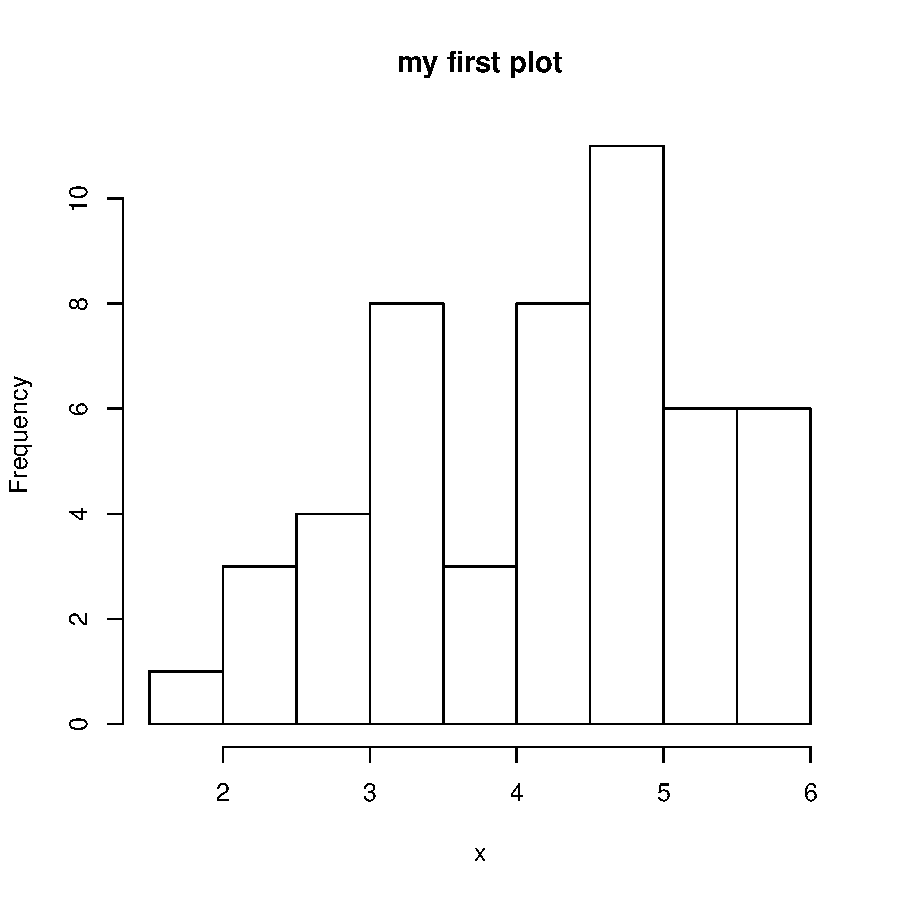
\includegraphics{Lab0-firstsessionplot}
\end{center}

% subsubsection example_1 (end)

\subsubsection{Tab completion} % (fold)
\label{ssub:tab_completion}
\begin{itemize}
    \item function names
    \item arguments
    \item file names
\end{itemize}
% subsubsection tab_completion (end)

\subsubsection{History} % (fold)
\label{ssub:history}
\begin{itemize}
    \item up, down arrow
    \item command `history'
    \item file `.Rhistory'
\end{itemize}

% subsubsection history (end)

\subsubsection{Prompt} % (fold)
\label{ssub:prompt}
\begin{itemize}
    \item Standard
    \item Continuation
    \item Other
\end{itemize}

% subsubsection prompt (end)


\subsubsection{Getting help}

\subsubsection{Help browser} % (fold)
\label{ssub:help_browser}
\begin{itemize}
    \item `?' command
    \item \texttt{help.search(\emph{command})}
    \item \texttt{help.start()}
\end{itemize}


% subsubsection help_browser (end)

\subsubsection{Examples} % (fold)
\label{ssub:examples}

\begin{itemize}
    \item \texttt{example(\emph{function})}
    \item \texttt{data}
\end{itemize}

% subsubsection examples (end)

\subsection{Session} % (fold)
\label{sub:session}

\subsubsection{Saving} % (fold)
\label{ssub:saving}

\begin{itemize}
    \item \texttt{save.image}
    \item \texttt{save}
    \item \texttt{load}
    \item \texttt{history}
\end{itemize}


% subsubsection saving (end)

\subsubsection{Quitting} % (fold)
\label{ssub:quitting}

\begin{itemize}
    \item \texttt{q()}
    \item saving/restoring session
    \item dumping
\end{itemize}

% subsubsection quitting (end)

\subsubsection{Aborting} % (fold)
\label{ssub:aborting}

\begin{itemize}
    \item C-c
    \item Esc
    \item kill
\end{itemize}

% subsubsection aborting (end)

% subsection session (end)

\section{Exploring \emph{R}} % (fold)
\label{sec:exploring_r}

\subsection{Example 2: Calculator} % (fold)
\label{sub:example_2_calculator}

\begin{Schunk}
\begin{Sinput}
> # Arithmetic
> 3 / 5
\end{Sinput}
\begin{Soutput}
[1] 0.6
\end{Soutput}
\begin{Sinput}
> 301 + 50000003
\end{Sinput}
\begin{Soutput}
[1] 50000304
\end{Soutput}
\begin{Sinput}
> 0.0005 * 0.0001
\end{Sinput}
\begin{Soutput}
[1] 5e-08
\end{Soutput}
\begin{Sinput}
> -0.0001 ** 9
\end{Sinput}
\begin{Soutput}
[1] -1e-36
\end{Soutput}
\begin{Sinput}
> -0.0001 ^ 9
\end{Sinput}
\begin{Soutput}
[1] -1e-36
\end{Soutput}
\begin{Sinput}
> ## exponentiation can be represented with either ** or ^
> 3 + 5 * 2
\end{Sinput}
\begin{Soutput}
[1] 13
\end{Soutput}
\begin{Sinput}
> (3 + 5) * 2
\end{Sinput}
\begin{Soutput}
[1] 16
\end{Soutput}
\begin{Sinput}
> ## special operations are called by name
> sin(3)
\end{Sinput}
\begin{Soutput}
[1] 0.14112
\end{Soutput}
\begin{Sinput}
> sqrt(5)
\end{Sinput}
\begin{Soutput}
[1] 2.236068
\end{Soutput}
\begin{Sinput}
> ## complex numbers are supported when written as x + yi
> -1 + 0i
\end{Sinput}
\begin{Soutput}
[1] -1+0i
\end{Soutput}
\begin{Sinput}
> sqrt(-1 + 0i)
\end{Sinput}
\begin{Soutput}
[1] 0+1i
\end{Soutput}
\begin{Sinput}
> ## constants can be called by name or expression (varies)
> pi
\end{Sinput}
\begin{Soutput}
[1] 3.141593
\end{Soutput}
\begin{Sinput}
> exp(1)
\end{Sinput}
\begin{Soutput}
[1] 2.718282
\end{Soutput}
\end{Schunk}


% subsection example_2_calculator (end)

\subsection{Example 3: Variables} % (fold)
\label{sub:example_3_variables}
\begin{itemize}
    \item letters, numbers, underscores, `.'
    \item convention
    \item reserved
\end{itemize}
\begin{center}
    \begin{tabular}{c|c}
        if & TRUE \\
        else & FALSE \\
        repeat & NULL \\
        while & Inf \\
        function & NaN \\
        for & NA \\
        in & NA\_integer\_ \\
        next & NA\_real\_ \\
        break & NA\_complex\_ \\
    \end{tabular}
\end{center}
% subsection example_3_variables (end)
\begin{Schunk}
\begin{Sinput}
> x <- 1:20
> y <-  x + (x/4 - 2)^3 + rnorm(20, sd=3)
> names(y) <- paste("O",x,sep=".")
> ww <- rep(1,20); ww[13] <- 0
> summary(lmxy <- lm(y ~ x + I(x^2)+I(x^3) + I((x-10)^2), weights = ww), cor = TRUE)
\end{Sinput}
\begin{Soutput}
Call:
lm(formula = y ~ x + I(x^2) + I(x^3) + I((x - 10)^2), weights = ww)

Residuals:
    Min      1Q  Median      3Q     Max 
-5.8699 -0.7917 -0.1534  1.3804  3.6724 

Coefficients: (1 not defined because of singularities)
               Estimate Std. Error t value Pr(>|t|)   
(Intercept)   -6.186503   2.877205  -2.150  0.04826 * 
x              3.294472   1.163444   2.832  0.01263 * 
I(x^2)        -0.287347   0.128323  -2.239  0.04072 * 
I(x^3)         0.012291   0.004052   3.033  0.00838 **
I((x - 10)^2)        NA         NA      NA       NA   
---
Signif. codes:  0 ‘***’ 0.001 ‘**’ 0.01 ‘*’ 0.05 ‘.’ 0.1 ‘ ’ 1 

Residual standard error: 2.63 on 15 degrees of freedom
Multiple R-squared: 0.9672,	Adjusted R-squared: 0.9606 
F-statistic: 147.4 on 3 and 15 DF,  p-value: 2.371e-11 

Correlation of Coefficients:
       (Intercept) x     I(x^2)
x      -0.90                   
I(x^2)  0.80       -0.97       
I(x^3) -0.73        0.93 -0.99 
\end{Soutput}
\begin{Sinput}
> variable.names(lmxy)
\end{Sinput}
\begin{Soutput}
[1] "(Intercept)" "x"           "I(x^2)"      "I(x^3)"     
\end{Soutput}
\begin{Sinput}
> variable.names(lmxy, full= TRUE)# includes the last
\end{Sinput}
\begin{Soutput}
[1] "(Intercept)"   "x"             "I(x^2)"        "I(x^3)"       
[5] "I((x - 10)^2)"
\end{Soutput}
\begin{Sinput}
> case.names(lmxy)
\end{Sinput}
\begin{Soutput}
 [1] "O.1"  "O.2"  "O.3"  "O.4"  "O.5"  "O.6"  "O.7"  "O.8"  "O.9"  "O.10"
[11] "O.11" "O.12" "O.14" "O.15" "O.16" "O.17" "O.18" "O.19" "O.20"
\end{Soutput}
\begin{Sinput}
> case.names(lmxy, full = TRUE)# includes the 0-weight case
\end{Sinput}
\begin{Soutput}
 [1] "O.1"  "O.2"  "O.3"  "O.4"  "O.5"  "O.6"  "O.7"  "O.8"  "O.9"  "O.10"
[11] "O.11" "O.12" "O.13" "O.14" "O.15" "O.16" "O.17" "O.18" "O.19" "O.20"
\end{Soutput}
\end{Schunk}

\subsubsection{Types} % (fold)
\label{ssub:types}
\begin{tabular}{r l l l}
    type & is a  & description  &  notes \\
    \hline
    integer & numeric & whole number  &       \\
    double  & numeric & floating point number       &       \\
    numeric &       &   any number    & base type       \\
    logical &        & TRUE or FALSE   & base type \\
    complex &       & complex number &       \\
    raw     &       & unparsed input string  &       \\
    character &       & letters and other characters &       \\
    list &       & collection of other objects &       \\
    expression &       & parsed but unevaluated input &       \\
    name     &       & character string referencing an object &       \\
    symbol &       & character string referencing an object  &       \\
    function (closure) &   & a function  &       \\
    pairlist &       & deprecated linked-list structure &       \\
    promise &       & reference to an expression whose evaluation & \\
    & & is delayed by \emph{lazy evaluation} but which is treated as being a value &       \\
\end{tabular}

% subsubsection types (end)

\subsubsection{Vectors and Matrices} % (fold)
\label{ssub:vectors}

\begin{Schunk}
\begin{Sinput}
> x <- 200
> half.x <- x/2
> threshold <- 95.0
> age <- c(15, 19, 30)
> age[2]      ## [] for accessing element.
\end{Sinput}
\begin{Soutput}
[1] 19
\end{Soutput}
\begin{Sinput}
> length(age) ## () for calling function.
\end{Sinput}
\begin{Soutput}
[1] 3
\end{Soutput}
\begin{Sinput}
> y <- c(10, 20, 40)
> y[2]
\end{Sinput}
\begin{Soutput}
[1] 20
\end{Soutput}
\begin{Sinput}
> length(y)
\end{Sinput}
\begin{Soutput}
[1] 3
\end{Soutput}
\begin{Sinput}
> x <- 5
> length(x)
\end{Sinput}
\begin{Soutput}
[1] 1
\end{Soutput}
\begin{Sinput}
> y <- c(20, 49, 16, 60, 100)
> min(y)
\end{Sinput}
\begin{Soutput}
[1] 16
\end{Soutput}
\begin{Sinput}
> range(y)
\end{Sinput}
\begin{Soutput}
[1]  16 100
\end{Soutput}
\begin{Sinput}
> sqrt(y)
\end{Sinput}
\begin{Soutput}
[1]  4.472136  7.000000  4.000000  7.745967 10.000000
\end{Soutput}
\begin{Sinput}
> log(y)
\end{Sinput}
\begin{Soutput}
[1] 2.995732 3.891820 2.772589 4.094345 4.605170
\end{Soutput}
\begin{Sinput}
> x <- seq(from=1, to=9, by=2)
> y <- seq(from=2, by=7, length=3)
> z <- 4:8
> a <- seq.int(5)                ## fast for integers
> b <- c(3, 9, 2)
> d <- c(a, 10, b)
> e <- rep( c(1,2), 3)
> f <- integer(7)
\end{Sinput}
\end{Schunk}

\begin{Schunk}
\begin{Sinput}
> x <- 1:6
> is.matrix(x)
\end{Sinput}
\begin{Soutput}
[1] FALSE
\end{Soutput}
\begin{Sinput}
> dim(x) <- c(2,3)
> is.matrix(x)
\end{Sinput}
\begin{Soutput}
[1] TRUE
\end{Soutput}
\begin{Sinput}
> x
\end{Sinput}
\begin{Soutput}
     [,1] [,2] [,3]
[1,]    1    3    5
[2,]    2    4    6
\end{Soutput}
\begin{Sinput}
> dim(x)
\end{Sinput}
\begin{Soutput}
[1] 2 3
\end{Soutput}
\begin{Sinput}
> x[2,2]
\end{Sinput}
\begin{Soutput}
[1] 4
\end{Soutput}
\begin{Sinput}
> x[1,]                           ## extracting values.
\end{Sinput}
\begin{Soutput}
[1] 1 3 5
\end{Soutput}
\begin{Sinput}
> x[1:2, 2:3]
\end{Sinput}
\begin{Soutput}
     [,1] [,2]
[1,]    3    5
[2,]    4    6
\end{Soutput}
\begin{Sinput}
> x[,2]                           ## not column vector!
\end{Sinput}
\begin{Soutput}
[1] 3 4
\end{Soutput}
\begin{Sinput}
> x[,2,drop=F]                    ## gotcha!
\end{Sinput}
\begin{Soutput}
     [,1]
[1,]    3
[2,]    4
\end{Soutput}
\begin{Sinput}
> m <- matrix( floor(runif(6, max=50)), nrow=3) ##ncol=2
> x <- rbind( c(1,4,9), c(2,6,8), c(3,2,1))
> y <- cbind( c(1,2,3), 5, c(4,5,6))  # recycling again
> x <- matrix(1:4, 2,2)
> i <- diag(2) ## 2x2 identity matrix
> x %*% i      ## should be x
\end{Sinput}
\begin{Soutput}
     [,1] [,2]
[1,]    1    3
[2,]    2    4
\end{Soutput}
\begin{Sinput}
> x  *  i      ## not x!
\end{Sinput}
\begin{Soutput}
     [,1] [,2]
[1,]    1    0
[2,]    0    4
\end{Soutput}
\end{Schunk}
% subsubsection vectors (end)

\subsection{Example 4: Functions} % (fold)
\label{sub:example_4_functions}

% subsection example_4_functions (end)

\subsection{Miscellany} % (fold)
\label{sub:miscellany}

% subsection miscellany (end)



% section exploring_r (end)

\section{Source files} % (fold)
\label{sec:source_files}

\subsection{Overview} % (fold)
\label{sub:overview_s}

% subsection overview_s (end)

\subsection{Functions} % (fold)
\label{sub:functions}

% subsection functions (end)

\subsection{Scripts} % (fold)
\label{sub:scripts}

% subsection scripts (end)

\subsection{Style} % (fold)
\label{sub:style}

\subsubsection{Conventions} % (fold)
\label{ssub:conventions}

% subsubsection conventions (end)

\subsubsection{Comments} % (fold)
\label{ssub:comments}

% subsubsection comments (end)

\subsubsection{White space} % (fold)
\label{ssub:white_space}

% subsubsection white_space (end)

% subsection style (end)

% section source_files (end)

\section{Plotting} % (fold)
\label{sec:plotting}

\begin{center}
\begin{Schunk}
\begin{Sinput}
> x <- seq(from=0, to=2*pi, len=1000)
> y <- cos(2*x)
> ## just provide data; sensible labelling
> plot(x,y)
\end{Sinput}
\end{Schunk}
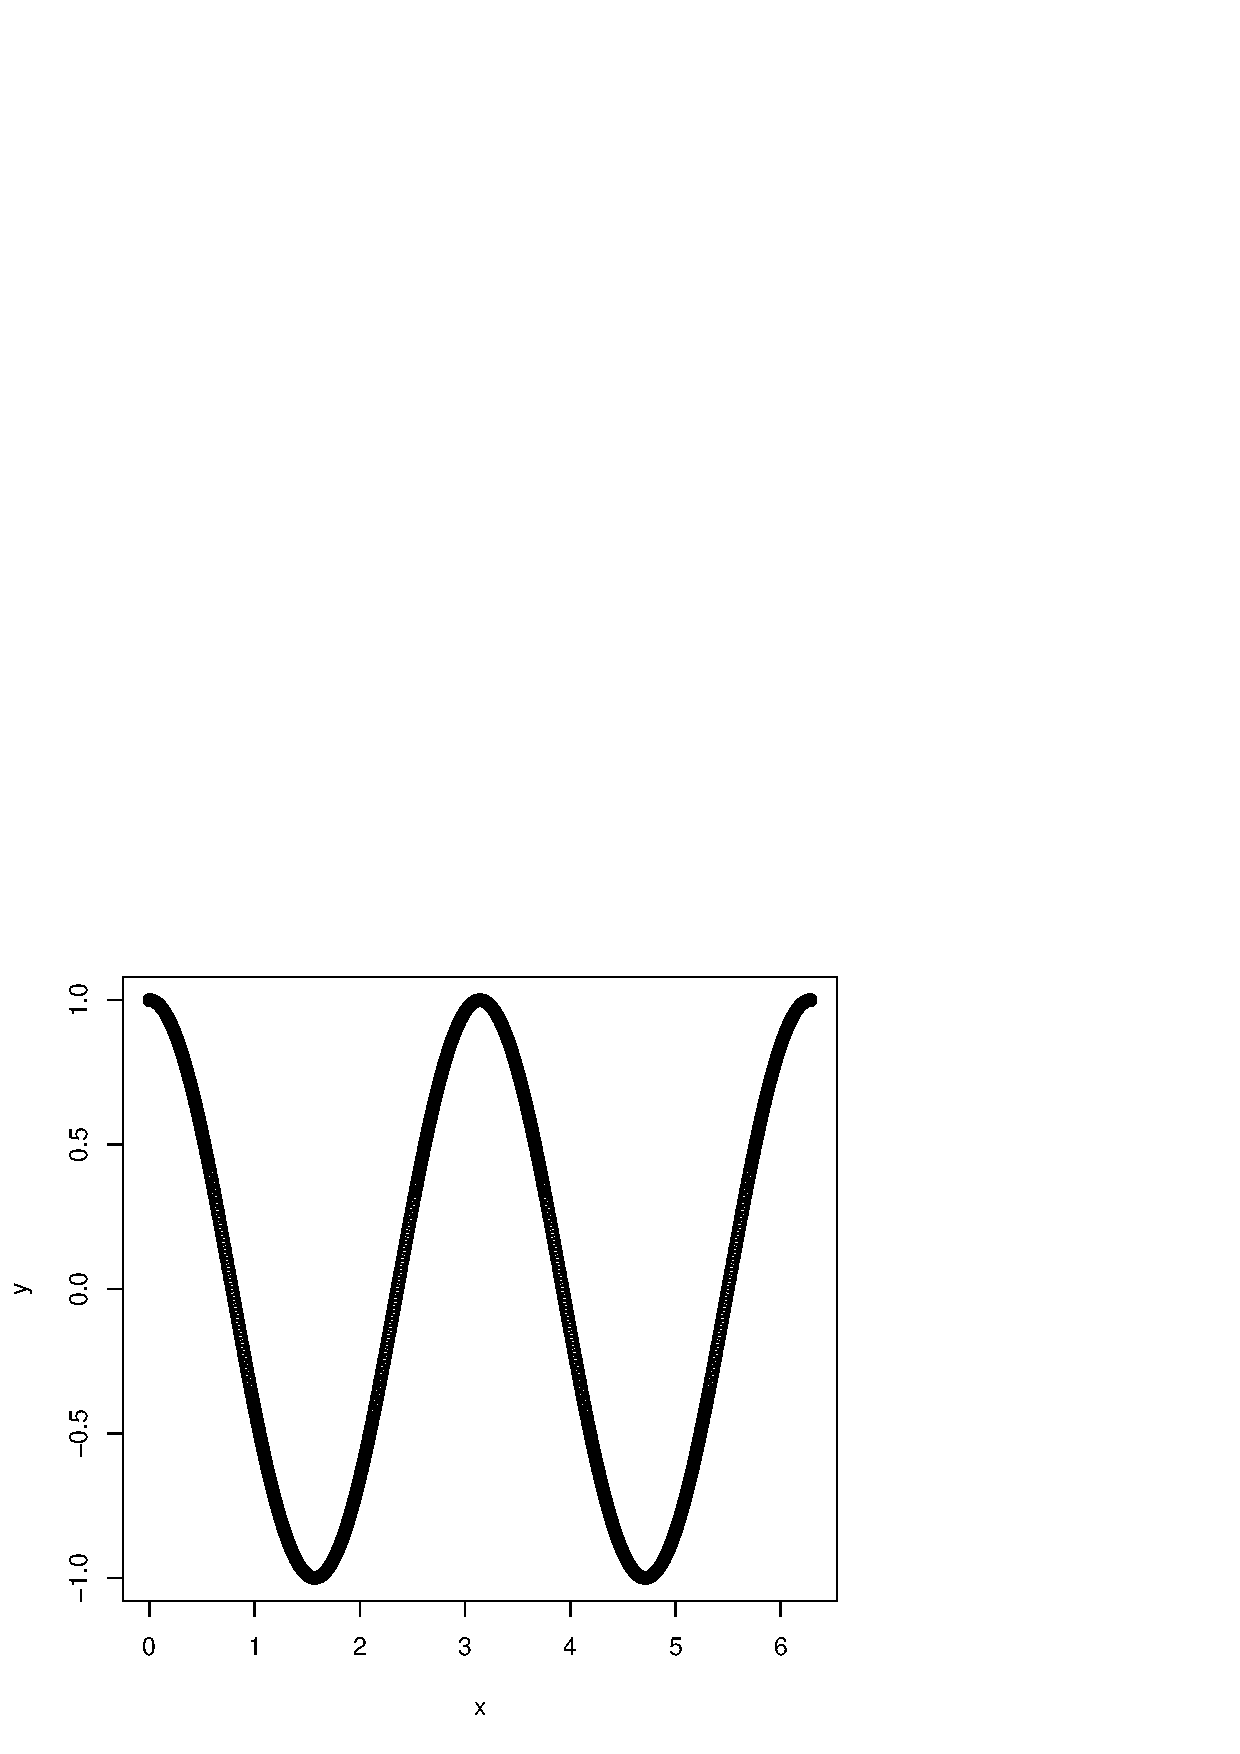
\includegraphics{Lab0-plotting_1}
\end{center}

\begin{center}
\begin{Schunk}
\begin{Sinput}
> ## Expand on previous plot ...
> plot(x,y, main='cos(2x)', type='l', lty=1, bty='n')
> y2 <- sin(2*x)
> lines(x,y2, main='sin(2x)', type='l', lty=2)
> same <- which( abs(y - y2) < 0.01)
> points(x[same], y[same], pch=19, col='red', cex=3)
> legend('bottomright', c("cos(2x)", "sin(2x)"),
+        lty=c(1,2))
\end{Sinput}
\end{Schunk}
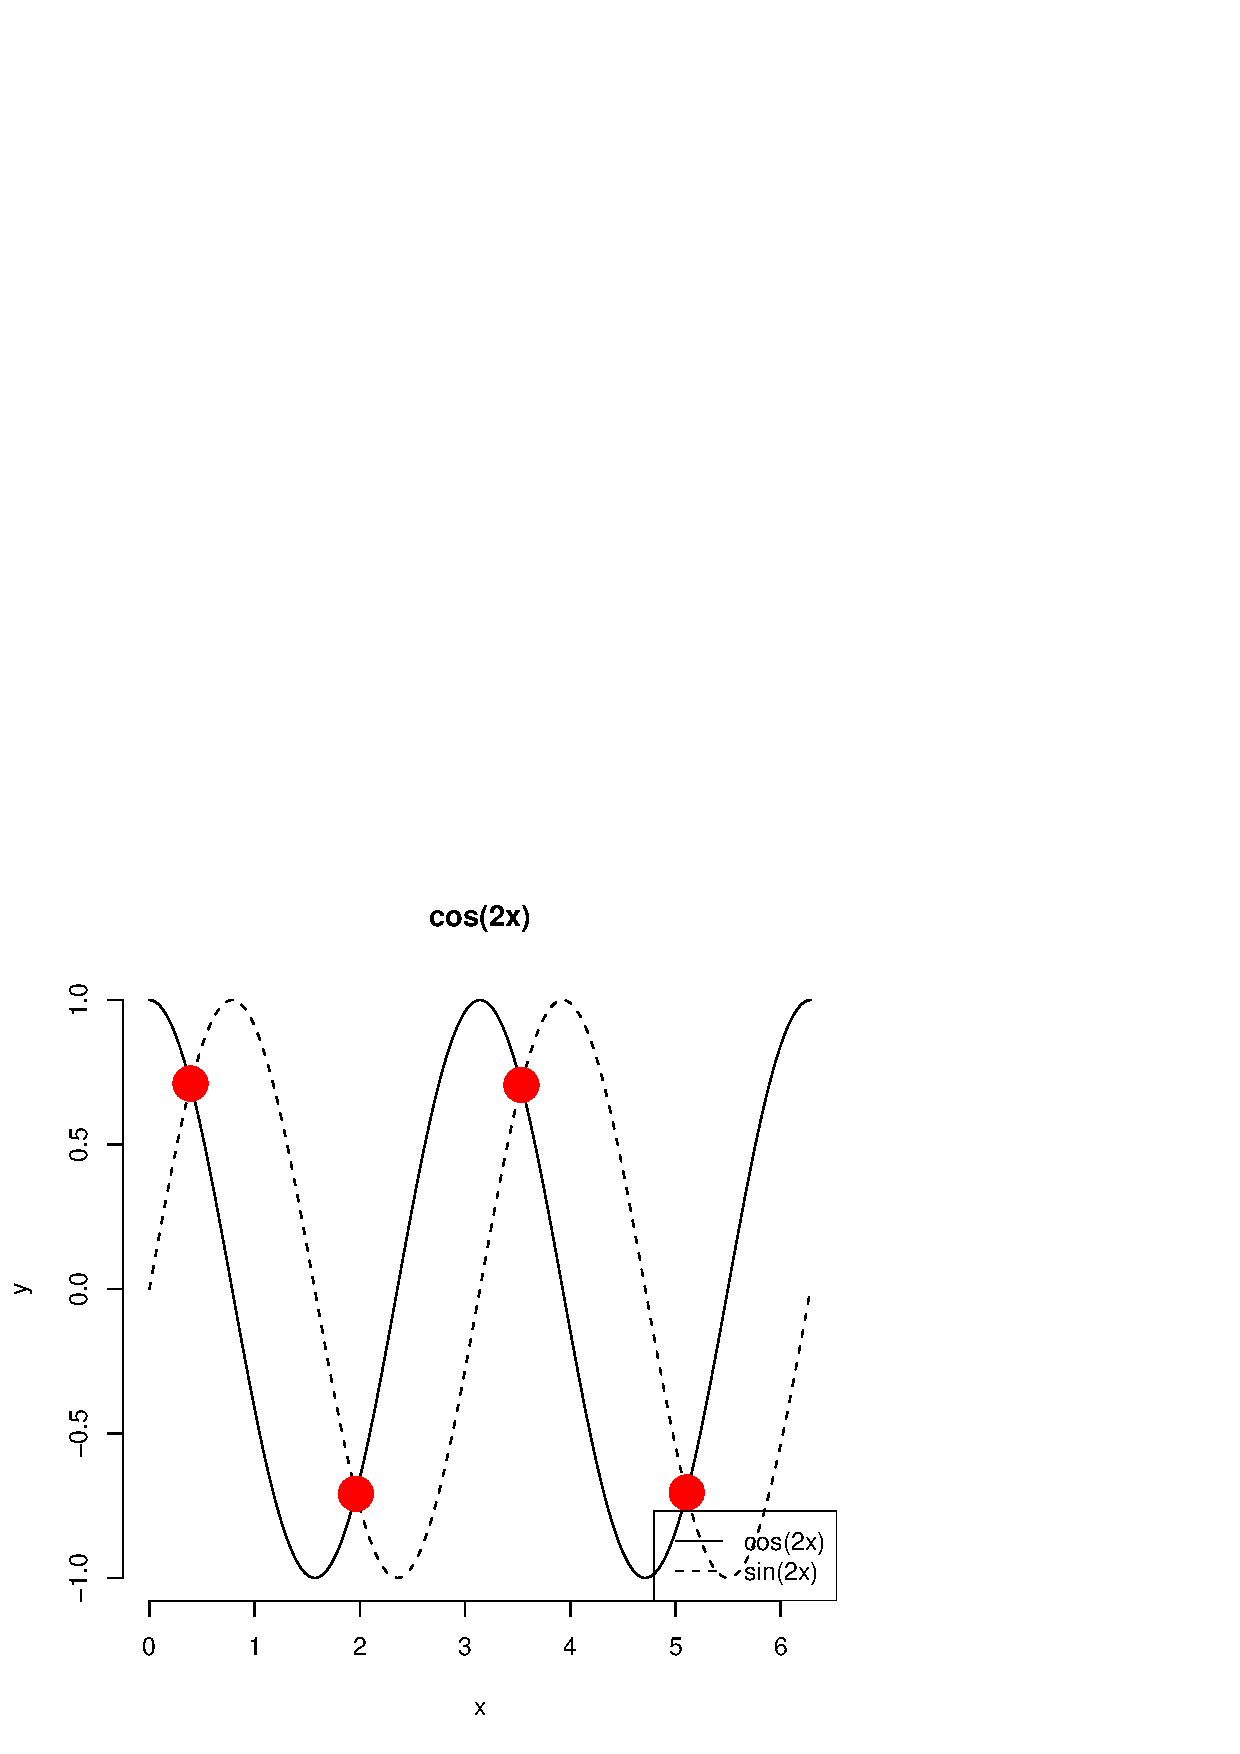
\includegraphics{Lab0-plotting_2}
\end{center}
% section plotting (end)


\bibliographystyle{plain}
\bibliography{}
\end{document}
